\section{\large Исследовательская часть}
\label{cha:research}

В данном разделе будут приведены примеры работы разработанной программы и поставлен эксперимент по исследованию зависимости времени обработки запроса в зависимости от количества полей таблиц. Результаты иссследования позволят точнее определять основные требования к базе данных при её выборе для проектирования системы, тем самым облегчая процесс выбора наиболее подходящей для конкретной задачи СУБД.	

%\subsection{Результаты разработки}

\subsection{Описание интерфейса}

В основной части страницы находятся методы API, а также их особенности (тип метода, адрес методы, структура, которую метод использует). Часть таких методов приведена на рисунке \ref{fig:interface-1}). 
\begin{figure}[h]
	\centering
	\captionsetup{justification=centering}
	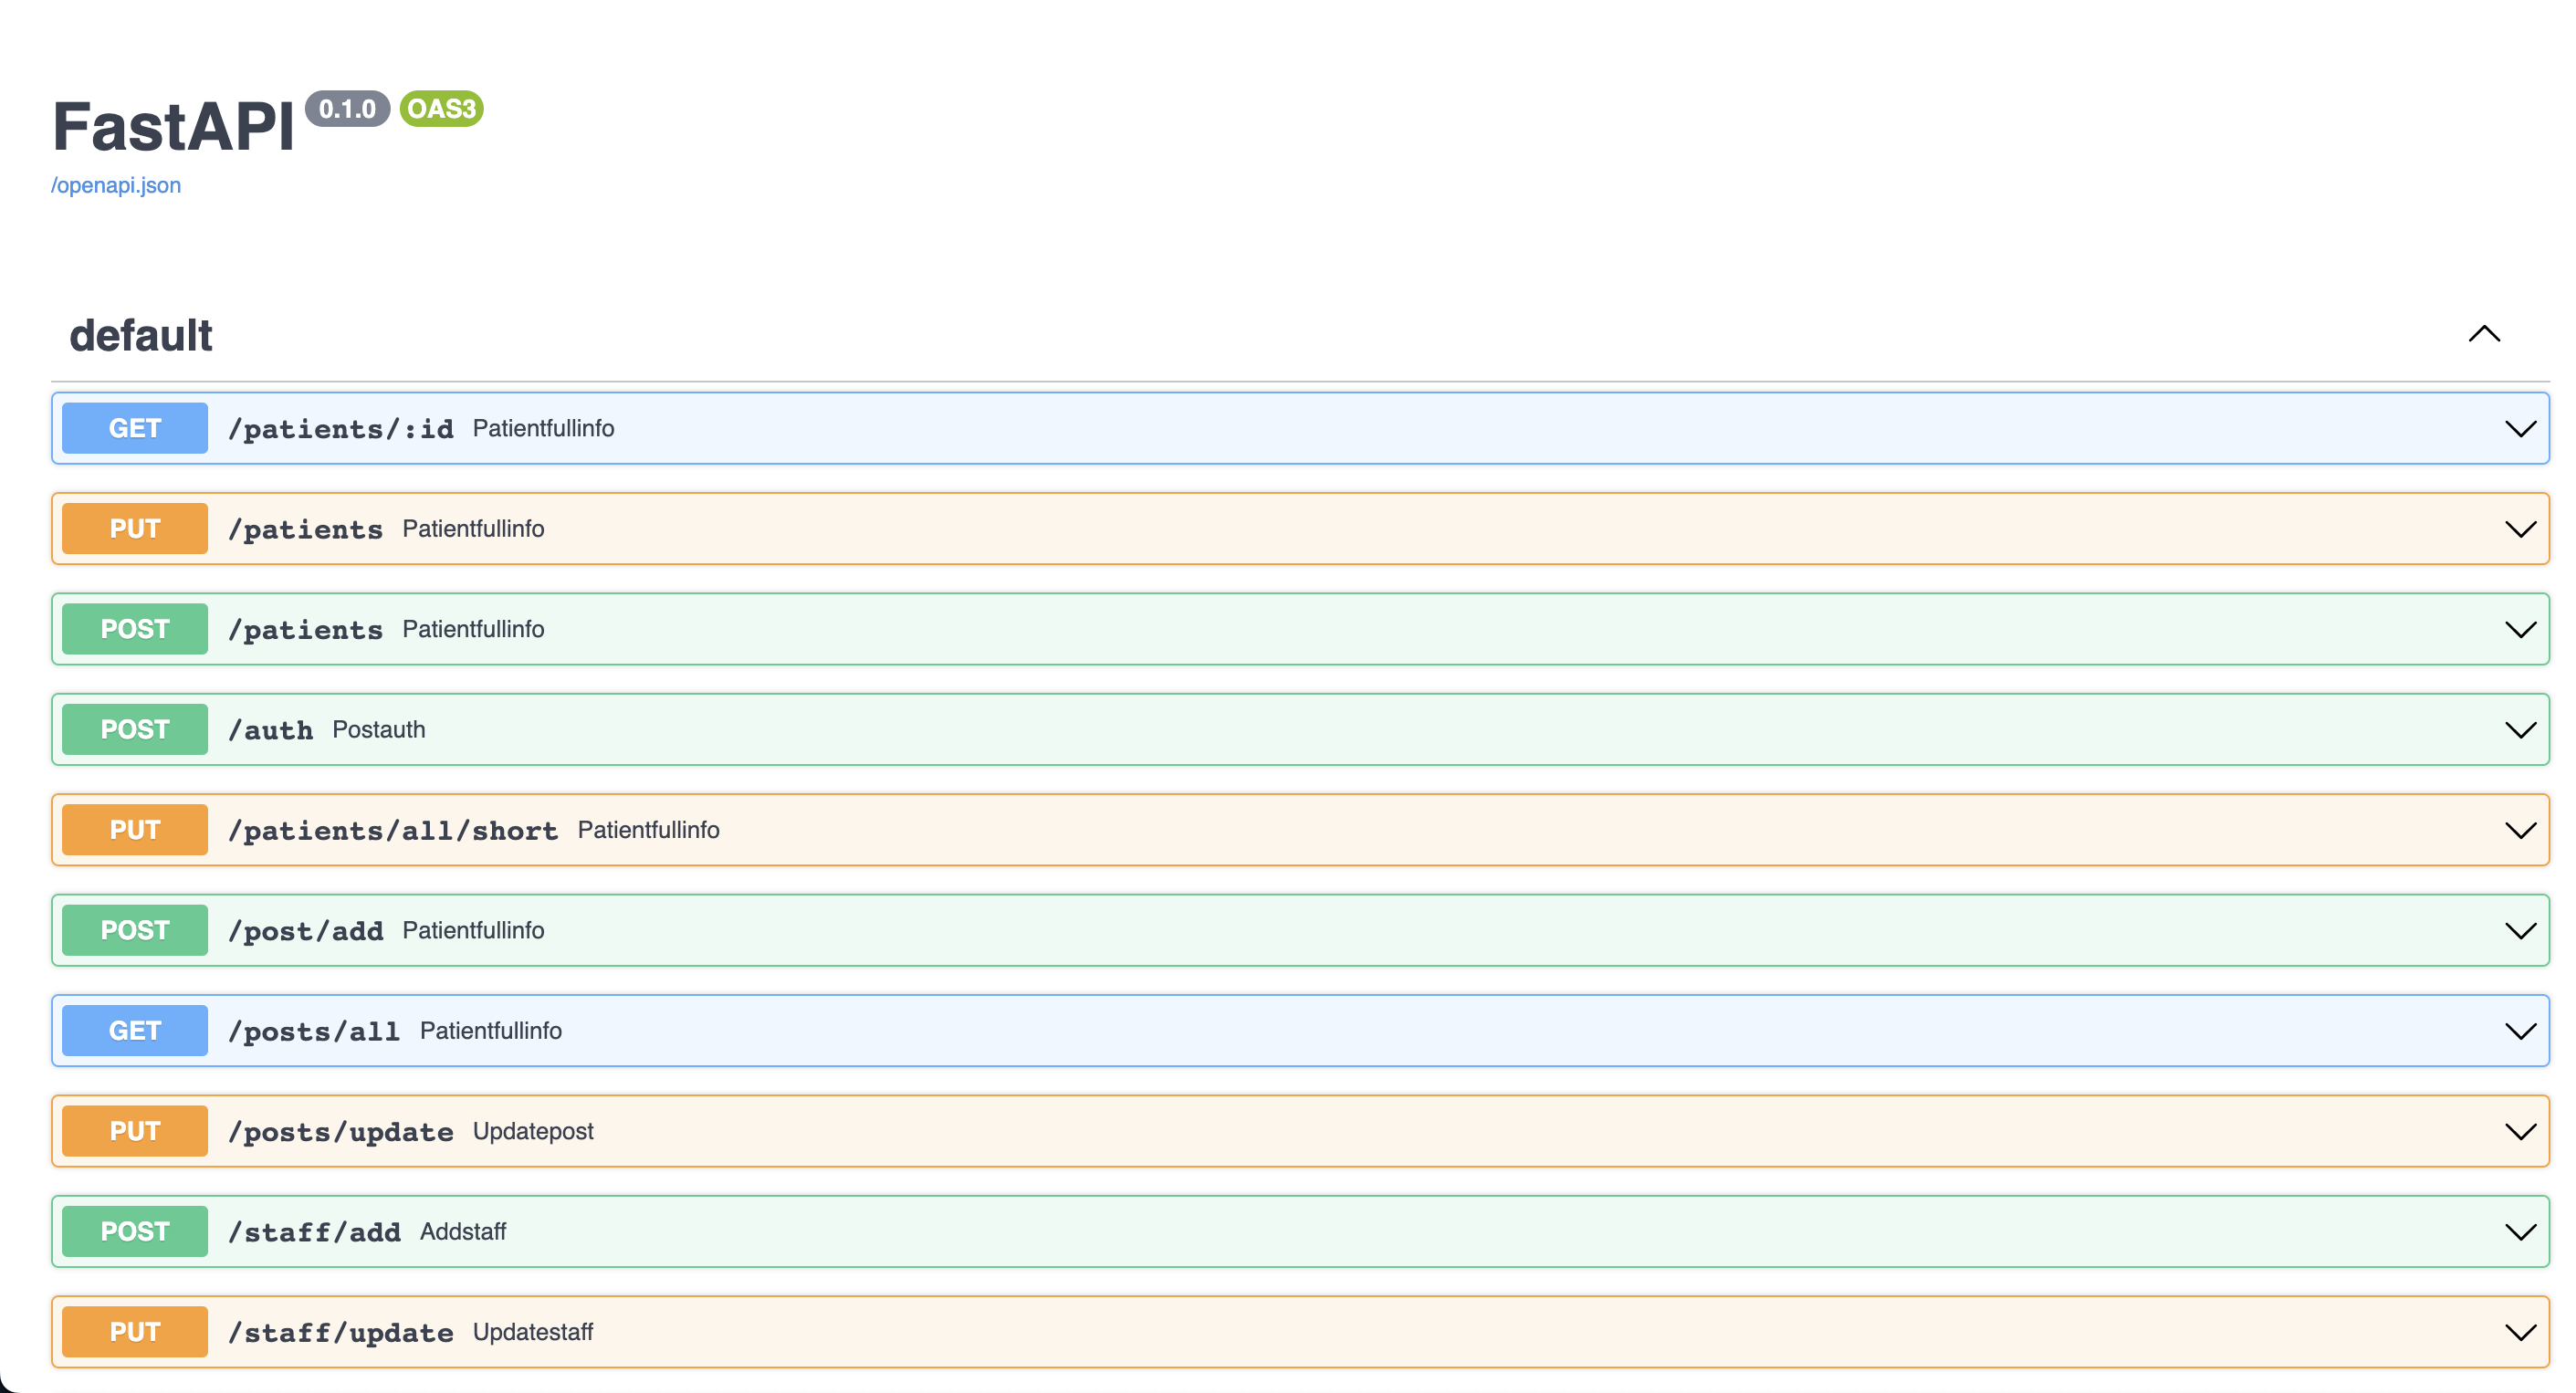
\includegraphics[width=170mm]{img/interface.png}
	\caption{Интерфейс программы: методы API}
	\label{fig:interface-1}
\end{figure}

По нажатию на элемент каждого метода появляется подробное описание: какие данные метод принимает на вход, какие параметры являются обязательными, а какие опциональными, структуры какого вида возвращает и в каком виде, что возвращает в случае ошибки (рисунок \ref{fig:interface-2}).
\begin{figure}[h]
	\centering
	\captionsetup{justification=centering}
	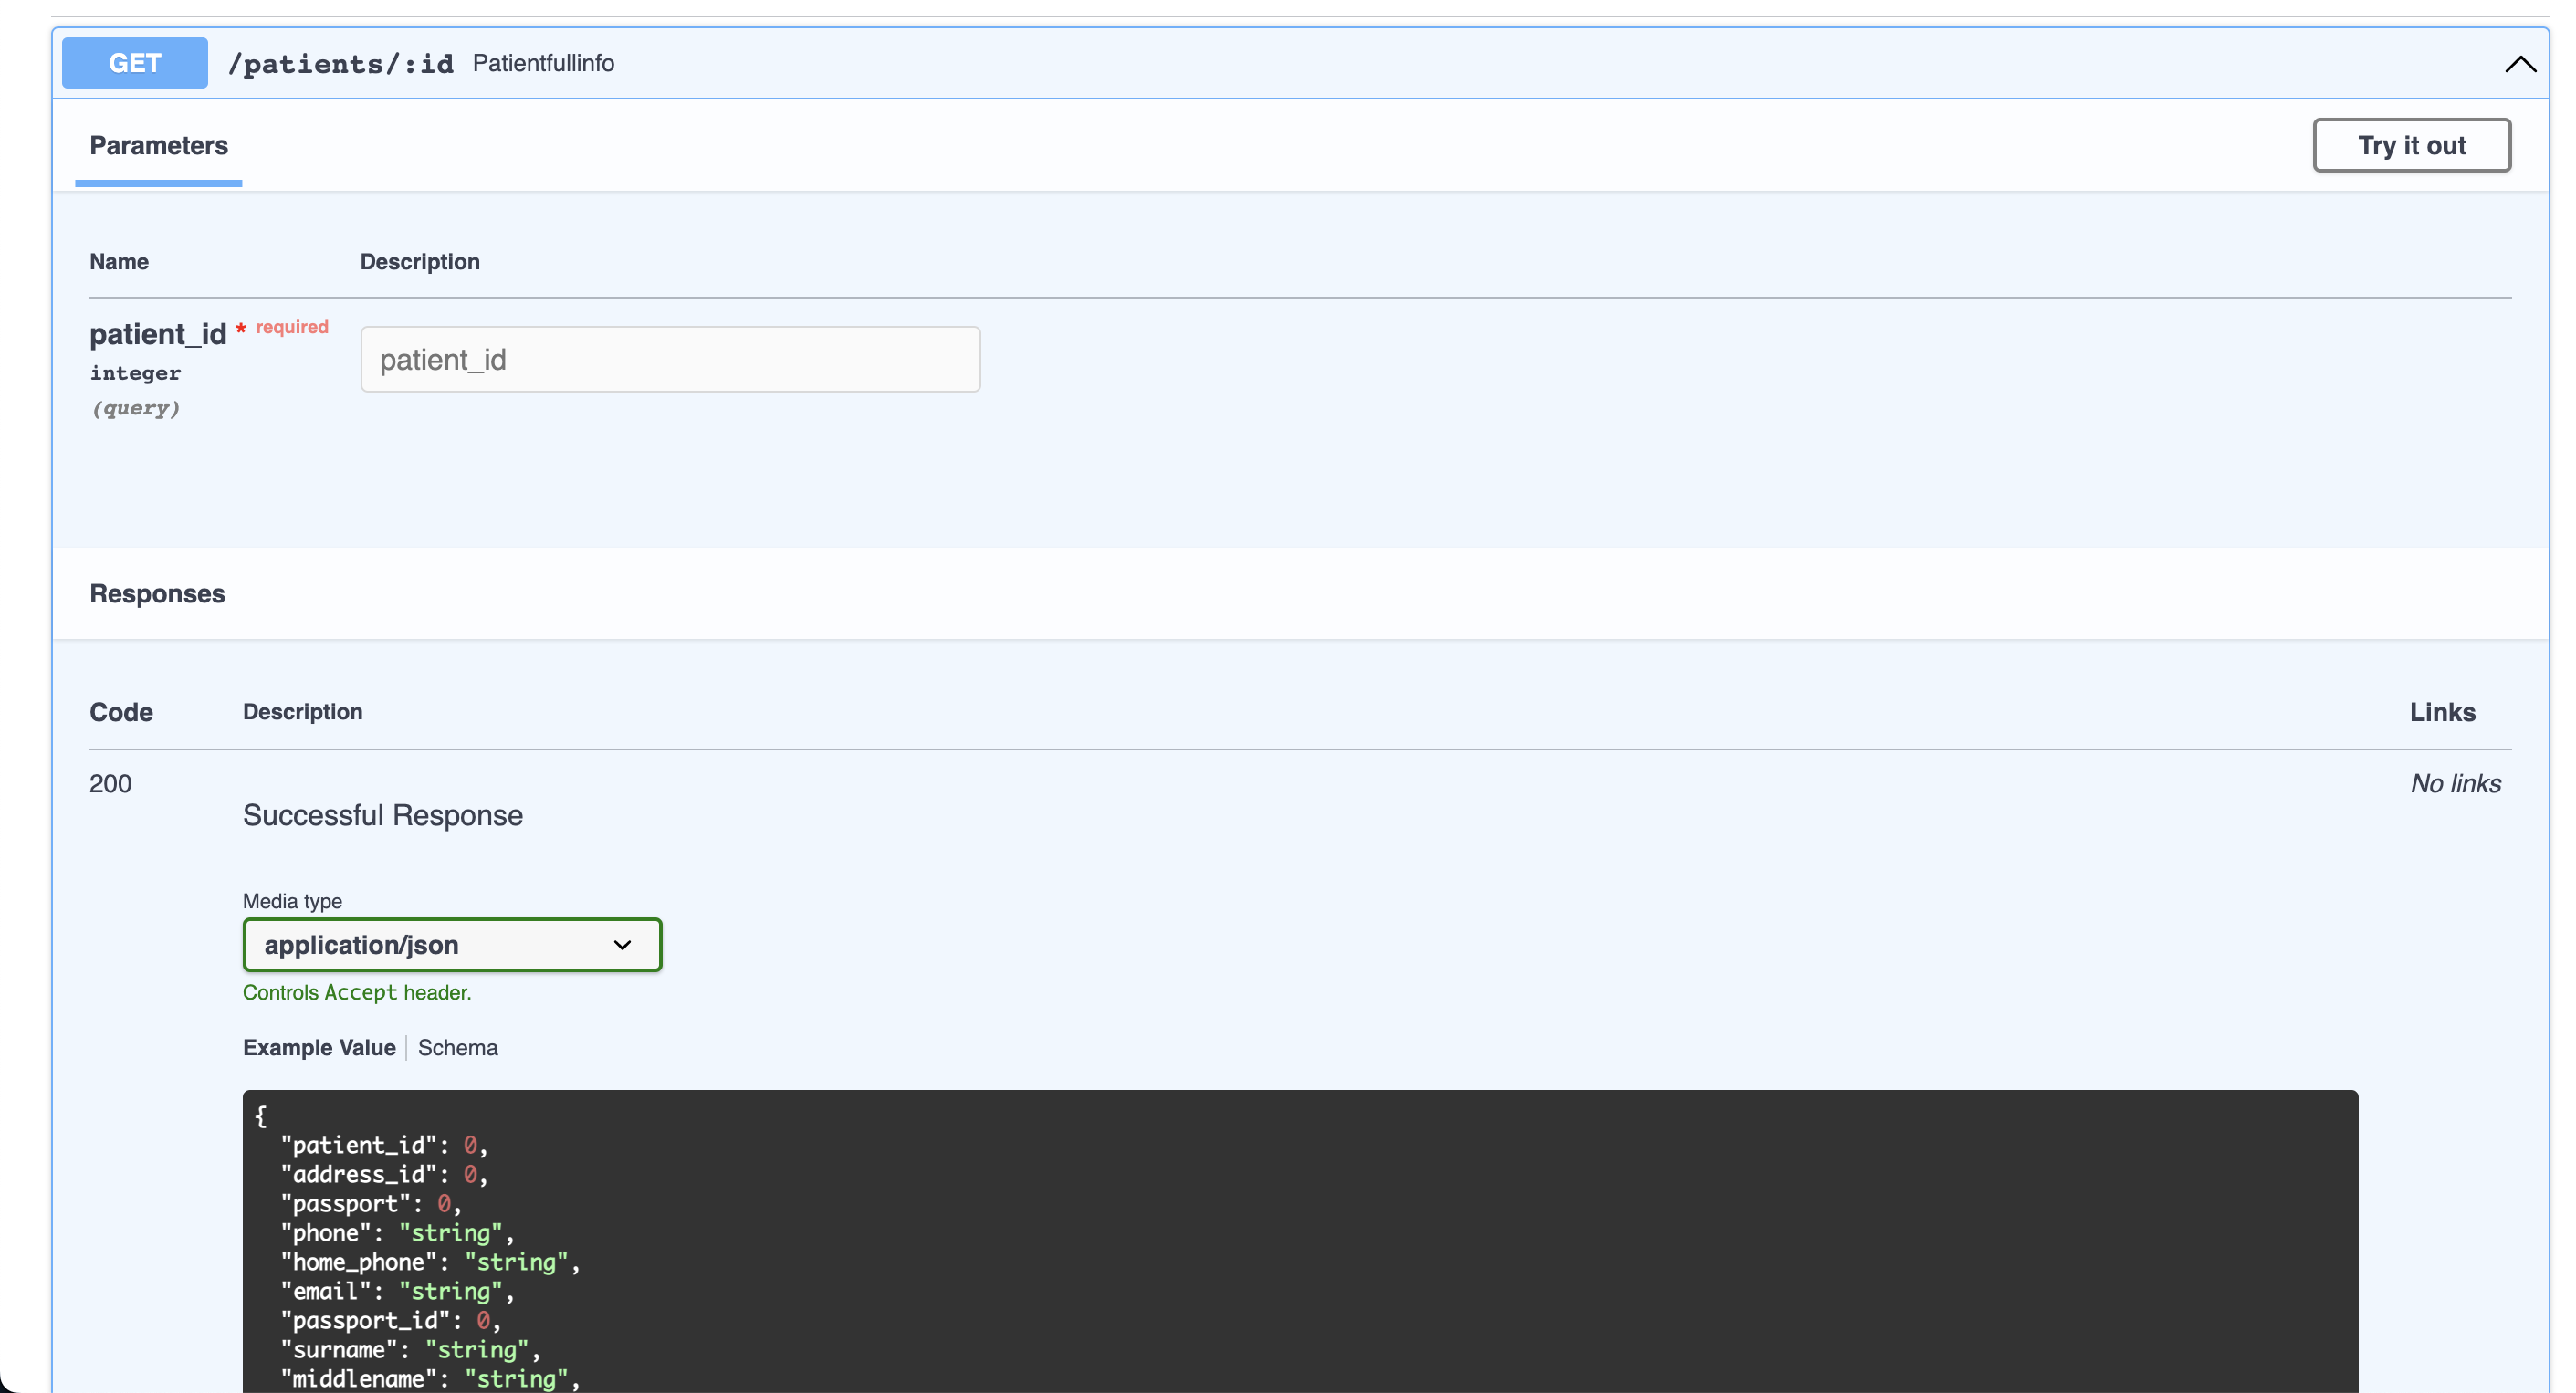
\includegraphics[width=170mm]{img/interface-2.png}
	\caption{Интерфейс программы: подробное описание метода API}
	\label{fig:interface-2}
\end{figure}


\subsection{Демонстрация работы программы}

На рисунках \ref{fig:example-1} -- \ref{fig:example-2} продемонстрирована работа программы на примере осуществления запроса для получения списка пациентов. Созданный интерфейс позволяет не толькоо просматривать методы API, как было показано выше, но и осуществлять отправку конкретных запросов.
При этом имеется возможность посмотреть результат запроса (его статус и заголовки, присланные данные), его адрес, а также получить команды для отправления эквивалентного запроса из командной строки.

\clearpage

\begin{figure}[h]
	\centering
	\captionsetup{justification=centering}
	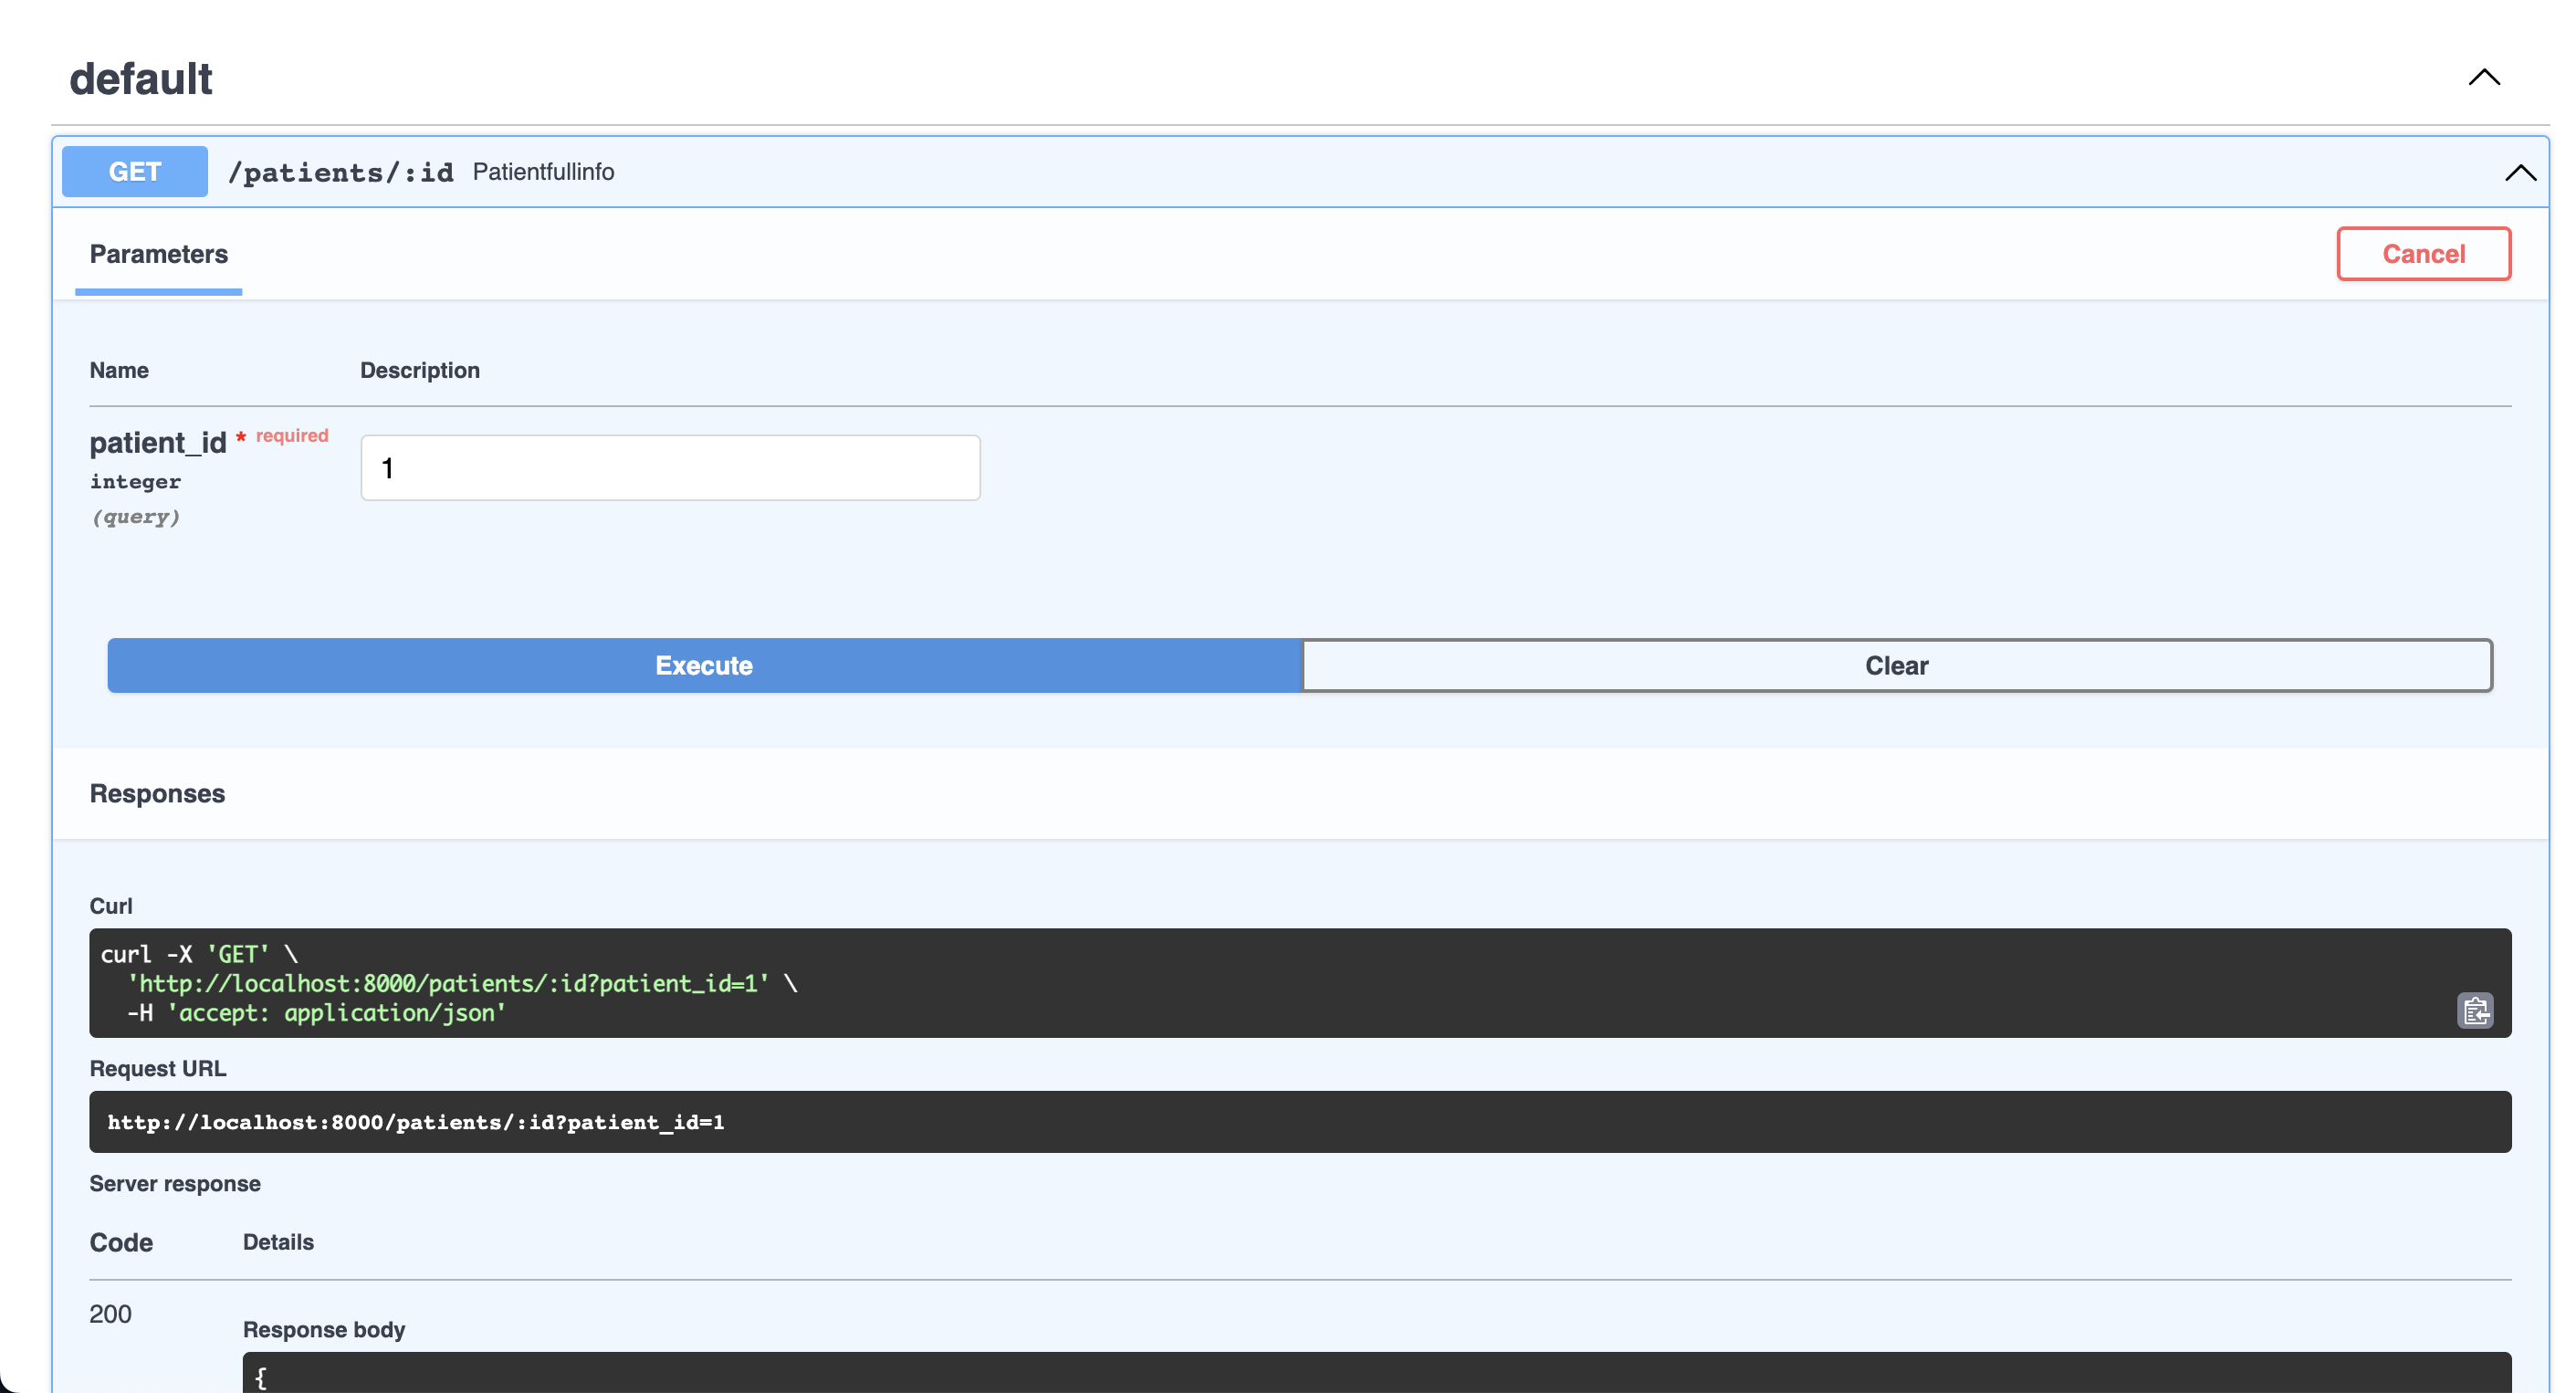
\includegraphics[width=152mm]{img/example-1.png}
	\caption{Демонстрация  работы  программы  (часть 1)}
	\label{fig:example-1}
\end{figure}

\begin{figure}[h]
	\centering
	\captionsetup{justification=centering}
 	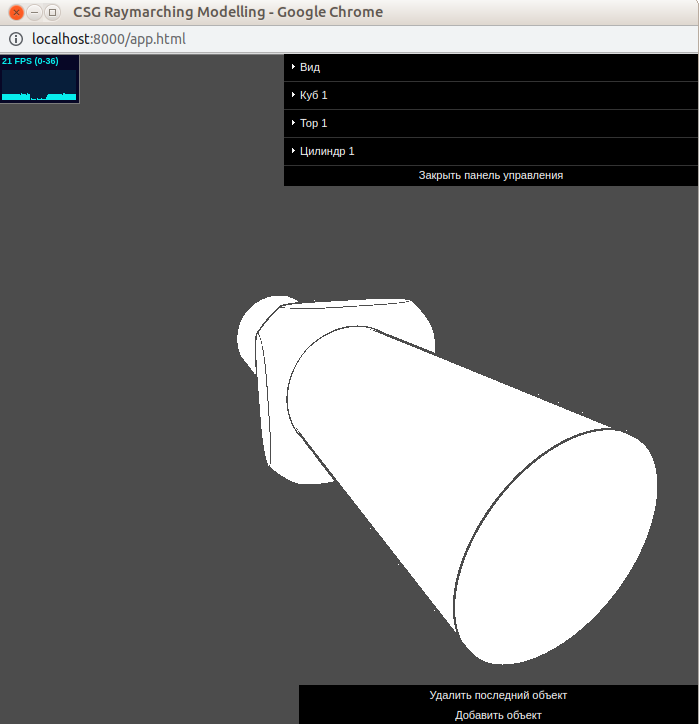
\includegraphics[width=152mm]{img/example-2.png}
	\caption{Демонстрация  работы  программы  (часть 2)}
	\label{fig:example-2}
\end{figure}

\subsection{Постановка эксперимента}

Целью эксперимента является сравнение времени обработки запроса \linebreak (GET, на примере получения списка пациентов) в зависимости от количества полей таблицы.

\clearpage

Технические характеристики устройства, на котором выполнялось тестирование:

\begin{itemize}[label=---]
	\item Операционная система: macOS Ventura 13.2.1 (22D68) \cite{macos};
	\item Память: 16 Гб с тактовой частотой 2133 МГц LPDDR3 \cite{memory};
	\item Процессор: Intel Core™ i7-8559U \cite{intel} с тактовой частотой  2.70 ГГц;
	\item Видеокарта: Intel Iris Plus Graphics 655 \cite{graphics} c объёмом памяти 1536 Мб.
\end{itemize}

Тестирование проводилось на ноутбуке, включенном в сеть электропитания. Во время тестирования ноутбук был нагружен только системой тестирования (работающим приложением) и системным окружением операционной системы.

\subsection{Сравнение времени обработки}

Результаты измерений  времени обработки запросов в зависимости от количества полей таблицы приведены в таблице \ref{tb:research_table} и на рисунке \ref{fig:graph}.

\begin{table}[H]
	\caption{Зависимость времени обработки запроса от количества полей в таблице}
	\begin{tabular}{|>{\centering\arraybackslash}p{0.3\textwidth} | >{\centering\arraybackslash}p{0.645\textwidth} | }
		\hline
		Количество полей & Время обработки, мс \\
		\hline
		10                   & ~~~~~1.10 \\
		100                  & ~~~~~2.07 \\
		1000                   & ~~~~~8.50\\
		10000              & ~~~~80.43 \\
		100000                   & ~~946.73\\
		1000000     & 8780.69 \\
		\hline
	\end{tabular}
	\label{tb:research_table}
\end{table}

\clearpage

\begin{figure}[h]
	\centering
	\captionsetup{justification=centering}
	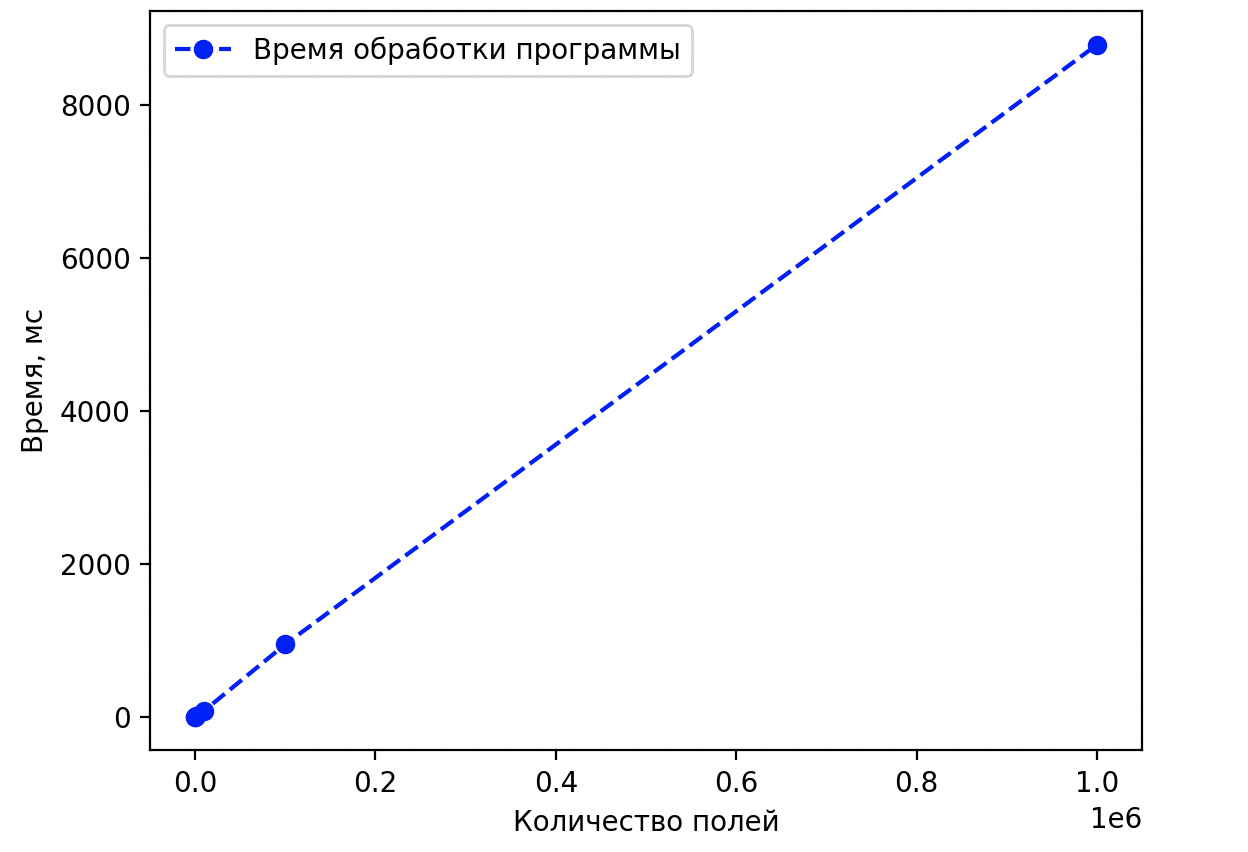
\includegraphics[width=130mm]{img/graph.png}
	\caption{Результаты замеров времени обработки запросов}
	\label{fig:graph}
\end{figure}


Результаты тестирования приводят к выводу, что зависимость времени обработки запроса от количества полей таблицы имеет линейный характер.

\subsection*{Вывод}
В данном разделе были описаны элементы интерфейса и приведены примеры работы разработанной программы. 
Графический интерфейс предоставляет возможность просмотреть список методов реализовнного API и их подробные характеристики (тип метода, адрес, используемые структуры), а также отправить конкретный запрос, осуществив ввод необходимых аргументов.
Проведён эксперимент по исследованию зависимости времени обработки запроса от количества полей таблицы. 
Исходя из результатов тестирования, характер зависимости является линейным.




